\documentclass[a4paper,english,10pt]{article}


%Using Lines
\usepackage{algorithm}
\usepackage{algorithmic}
\usepackage{amsmath}
\usepackage{relsize}
\usepackage{amsfonts}
\usepackage{amssymb}
\usepackage{mathtools}
\usepackage{graphicx}
\usepackage{epsfig}
\usepackage{color}
\usepackage{mathtools}
\usepackage{tikz}
\usepackage{relsize}
\usepackage{float}
\usepackage{dsfont}
\usepackage{hyperref}
\usepackage[nameinlink]{cleveref}
\newcommand{\bigqm}[1][1]{\text{\larger[#1]{\textbf{?}}}}
\usepackage{tikz,fullpage}
\usetikzlibrary{arrows, petri, topaths}
\usepackage{tkz-berge}
\usepackage[position=top]{subfig}
\usepackage{verbatim}
\usepackage{amsthm}
\usepackage{pgf}
\usepackage{tikz}
\usepackage{fancyhdr, setspace, color, soul}
\usepackage{geometry,polyglossia,fontspec,csquotes, doi}
\usepackage{ucs}
\usepackage[utf8x]{inputenc}
% \usepackage[english,hebrew]{babel}
\usepackage{breqn}
\usepackage{mdframed}
\usepackage{dsfont}
\usepackage{tabularx}
\usepackage{xcolor}
\usepackage{xspace}
\usepackage{cjhebrew}
\usepackage{caption}
\usepackage{subcaption}
\usepackage{subfig}
\usepackage{ascii}
\usepackage{multirow}
\usepackage{xfrac}
\usetikzlibrary{arrows, automata, backgrounds,snakes}
\newfontfamily\hebrewfont{Times New Roman}[Script=Hebrew]

% define MACROS
\newcommand{\len}{15}
\newcommand{\LPart}{0.4}
\DeclarePairedDelimiter{\ceil}{\lceil}{\rceil}
\DeclarePairedDelimiter{\floor}{\lfloor}{\rfloor}
\newtheorem{theorem}{Theorem}[section]
\newtheorem{corollary}{Corollary}[theorem]
\newtheorem{lemma}[theorem]{Lemma}
\newtheorem*{remark}{Remark}
\newcounter{casenum}
\newenvironment{caseof}{\setcounter{casenum}{1}}{\vskip.5\baselineskip}
\newcommand{\case}[2]{\vskip.5\baselineskip\par\noindent {\bfseries Case \arabic{casenum}:} #1\\#2\addtocounter{casenum}{1}}
\newcommand\rob{\ensuremath{r}\xspace}
\newcommand\opp{\ensuremath{o}\xspace}
\newcommand{\w}{\ensuremath{W}\xspace}
\newcommand{\fcc}{\ensuremath{FCC}\xspace}
\newcommand{\gipc}{\ensuremath{GIPC}\xspace}
\newcommand{\cros}{\ensuremath{CROS}\xspace}
\newcommand{\coos}{\ensuremath{COS}\xspace}
\newcommand{\gn}{\ensuremath{GN}\xspace}
\newcommand{\gf}{\ensuremath{GF}\xspace}
\newcommand{\go}{\ensuremath{GO}\xspace}
\DeclarePairedDelimiter\abs{\lvert}{\rvert}%
\DeclareMathOperator*{\argmax}{arg\,max} % Jan Hlavacek
\allowdisplaybreaks[2]
\newtheorem{definition}{Definition}
\def\checkmark{\tikz\fill[scale=0.4](0,.35) -- (.25,0) -- (1,.7) -- (.25,.15) -- cycle;}
\def\uncheckmark{$\mathbin{\tikz [x=1.4ex,y=1.4ex,line width=.2ex] \draw (0,0) -- (1,1) (0,1) -- (1,0);}$}
\newcommand{\Cross}{$\mathbin{\tikz [x=1.4ex,y=1.4ex,line width=.2ex, red] \draw (0,0) -- (1,1) (0,1) -- (1,0);}$}%

\makeatletter
\def\BState{\State\hskip-\ALG@thistlm}
\makeatother
% end


%%%%%% Latex Configuration
\renewcommand{\topfraction}{0.85}
\renewcommand{\textfraction}{0.1}
\renewcommand{\algorithmiccomment}[1]{// #1}
%%%%%
\long\def\symbolfootnote[#1]#2{\begingroup%
\def\thefootnote{\fnsymbol{footnote}}\footnote[#1]{#2}\endgroup}


%\setotherlanguage[numerals=western]{hebrew}
%\setdefaultlanguage{english}
\setmainlanguage{english}

\begin{document}
\begin{titlepage}
\begin{center}



\includegraphics[width=0.9\textwidth]{Images/logo.jpg}\\[1cm]
\textsc{\LARGE Bar Ilan University}\\[1.5cm]
\textsc{\Large M.Sc Proposal}\\[0.5cm]
%\hrule \\[0.4cm]
%{\huge \bfseries Speeding Frontier-Based Exploration by
%Using Semantic Labeling}\\[0.4cm]
%\hrule \\[1.5cm]

\hrule
{ \vspace{2 mm} }
{ \huge \bfseries Competitive Coverage}
{ \vspace{3 mm} }
\hrule
{ \vspace{8 mm} }

\hrule
{ \vspace{2 mm} }

{ \huge \bfseries  \huge \bfseries \<b`yyt hkyswy ht.hrwty> }
{ \vspace{3 mm} }
\hrule
{ \vspace{8 mm} }

% \author{Moshe N. Samson\\
% advised by Noa Agmon\\
% The MAVERICK Group, Computer Science Department\\
% Bar Ilan University\\
% Ramat Gan, Israel 52900\\
% \tt\small samson.moshe@gmail.com

%author and supervisor
\begin{minipage}{0.4\textwidth}
\begin{flushleft} \large
\emph{Author:}\\
Moshe N. Samson 

\end{flushleft}
\end{minipage}
\begin{minipage}{0.4\textwidth}
\begin{flushleft} \large
\emph{Supervisor:} \\
Dr. Noa Agmon
\end{flushleft}
\end{minipage}


\vfill


\large{The SMART Group, Computer Science Department\\
Bar Ilan University\\
Ramat Gan, Israel 52900\\
\tt\small samson.moshe@gmail.com}

\vfill

\today

\end{center}
\end{titlepage}

%opening
\title{Competitive Coverage}
\author{Moshe N. Samson\\
advised by Dr. Noa Agmon\\
The SMART Group, Computer Science Department\\
Bar Ilan University\\
Ramat Gan, Israel 52900\\
\tt\small samson.moshe@gmail.com
}

\tableofcontents
\maketitle

\section{Introduction}
The robotic coverage problem is one of the fundamental problems in robotic research, and as such has received considerable attention in the past two decades \cite{galceran2013survey}. The problem has its theoretical interest, but is of special interest due to its immediate applicability in real world settings, such as cleaning, coating, demining and search and rescue. 

In the original problem of robotic coverage, a robot's goal is to determine a path that will visit each point in a given area at least once, usually while minimizing the time for completion \cite{galceran2013survey}. The problem has been examined in different settings, for example offline vs. online coverage \cite{gabriely2001spanning,agmon2008giving}, where the environment map is given in advance or discovered during the execution (respectively), coverage with the presence of threats that might stop the robot \cite{yehoshua2014safest}, and continuous vs. discrete domains \cite{gabriely2001spanning,yang2004neural}. In the multi-robot coverage problem, the coverage is a collaborative effort: each point in the area should be visited at least once by some robot from the team, and the common goal is to minimize the maximal working time of some robot from the team. 

In this work we formally define a new variant of the coverage problem, {\em competitive coverage}, in which robots do not work collaboratively, but competitively. More formally, two robots, \rob and \opp, are to cover a given area represented as a grid, and our goal is to maximize the number of cells \rob covers first, before they are covered by \opp.

The problem can be classified as {\em symmetric} or {\em asymmetric}, which refers to wither \opp even knows about \rob's existence or not, regardless to what is the extent of such information. In this work we examine in depth the {\em asymmetric} variant of the problem, in which \opp operates without the knowledge of \rob's existence, and \rob knows it should compete with \opp. The problem is also modeled by the level of information one robot has on the other (beside its existence): initial location and strategy/coverage-path. We consider four different models: (i) \rob knows the initial location of \opp and its planned coverage path ; (ii) \rob knows only the path, but does not know \opp's initial location ; (iii) \rob knows \opp's initial location, but not its coverage path ; (iv) \rob does not know both \opp's path and its location.

Solving the competitive coverage problem, in some cases, is as computationally hard as solving the original coverage problem \cite{arkin2000approximation}. For the sake of the analysis, we consider environments in which an optimal coverage path can be computed in polynomial time, for example by using the Spanning-Tree Coverage Algorithm \cite{gabriely2001spanning}, which generates, cyclic coverage paths under some assumptions on the environment. 

We therefore present an optimal algorithm for \opp in the full-information case, and show that, surprisingly, having some information is equivalent (in the average case) to having no information at all. That is, if \rob has information only on \opp's location {\em or} on its path, its optimal behavior is exactly as if it does not know any of those. We support our theoretical analysis with ROS/Gazebo simulation, demonstrating our findings. 

\section{Background and Related Work}
The problem of single-robot coverage has been extensively discussed in the literature, and many approaches to coverage path planning have been developed though the years. In \cite{galceran2013survey} Galceran and Carreras offer a recent survey of coverage path planning methods.

The coverage problem can be classified as either offline or online. 
Online algorithms assumes zero or partial knowledge regarding the world to be covered, and the coverage-path is generated while advancing in that world. Conversely, Offline algorithms rely on stationary, known beforehand map of the world, and thus create the full coverage-path before even starting to move through it. In this work, we focus on offline coverage.

The coverage problem has been reduced to the traveling salesman problem \cite{arkin2000approximation}, and thus known to be $\mathcal{NP}$-complete even on simple graphs such as grid graphs \cite{papadimitriou1977euclidean}. However, there are known solutions to the coverage problem, that work even in linear time. For example, the offline algorithm STC, presented in \cite{gabriely2001spanning} has been proven to be optimal on discrete world, computes an optimal covering path in linear time $O(N)$, where $N$ is the number of cells comprising the approximate area. In our work we considered an approximate cellular decomposition (as explained in \cite{galceran2013survey}) into finite grid, and thus we know there exists an optimal coverage path which can be found in a linear time.

A considerable attention has been given in the literature also to the multi-robot variant of the coverage problem. In multi-robot coverage, multiple robots work in coordination in order to jointly cover an area. The robots can be with or without leader(s), relying on full or limited communication (e.g., \cite{agmon2008giving}), in online or offline manner \cite{agmon2008giving, de2005blind}.
In this work we do consider multiple (exactly 2) robots, but working noncooperately, one on each side.

Yehoshua et al. \cite{yehoshua2013robotic} recently introduced a new variant of the coverage problem, in which the covering robots operate in an adversarial environment, where threats exist and might stop the robot. Online algorithms for adversarial coverage were discussed in  \cite{yehoshua2015online}, and multi-robot algorithms for adversarial coverage were discussed in \cite{yehoshua2016multi}.
In this work other robots considered as competitors, and are not being a threat to our robot. %The robot does/doesn not have a behavior to meeting with its opponent, but in any case, it does not make it stop.

Another worth-mentioning niche relating to coverage is the patrolling task, in which the robot(s) are to repeatedly visit the area in order to monitor change in state. Most Patrol algorithms are either partition-based, where the area is divided into sub-areas, and each one is assigned to a robot (e.g., \cite{guo2004towards}, \cite{guo2004coverage}, \cite{jung2002tracking}), or are cyclic-based, where all robots travel through one cyclic path, coordinately \cite{chevaleyre2004theoretical}. 
In adversarial patrolling (\cite{agmon2011multi}, \cite{sless2014multi}, \cite{agmon2008multi}), there is an adversary trying to penetrate through the patrol path, undetected. In this work we consider competitors, where both are already in the area, and are trying to visit it as fast as possible. %Also, in patrolling, the enemy is trying (most of the time) to avoid from being detected, while in this work, the other opponent does not necessarily is trying to hide: its concern is different from the one in the Patrol problem.

Finally, the competitive problem is related to the foraging problem, which is searching, and when found, transporting objects to one or more collection points. In \cite{winfield2009foraging} we find a fairly extensive survey of the subject, including defining and describing the principles of foraging, presents the essentials design features that are a requirement for any foraging robot, and presents strategies for multi-robot foraging. \cite{winfield2009foraging} uses Finite-State-Machine to describe the states that constitute foraging. In our work, the robot does not need find anything, therefore there is not the notion of 'capacity' (that exists in foraging), and the choice to go back to certain points depends on the covering strategy assumptions (which, in our case, says that only position visited more than once is the initial position).

\section{Competitive Coverage: Definition}
Let \rob and \opp be two robots operating in an obstacle-free grid \w of size $N=m \times n$. Both robots move in the four basic directions (North, South, East, West). Consider \rob to be our robot-of-interest, and \opp to be the opponent. 
The goal of each robot is to cover the area, that is, find a path (denoted as the coverage path) that visits  each point in the area at least once. We define a coverage strategy of a robot as the coverage path, including the order of cells visited (specifically in a cyclic coverage path, the strategy indicates both the cells' ordering, and the direction of movement---clockwise or counterclockwise), or a behavior (for example: opponent chooses randomly, at each step, one of its four neighbors, and go there). We denote \rob's and \opp's strategies by $S_\rob,S_\opp\in \mathcal{S}$, respectively, where $\cal{S}$ stands for the possible strategies space. In the offline version of the competitive coverage problem, $S_\rob$ and $S_\opp$ are computed in advance (before the execution), and mostly consist of cells permutation, where in the online problem, the strategies are behaviors, able to adjust online to the environment.

\opp is covering \w using an optimal coverage strategy, that is, it follows a path guaranteeing coverage in minimal time (we based our experiments on the Spanning-Tree Coverage algorithm \cite{gabriely2001spanning}). \rob's goal is to cover as many cells as possible from \w {\em before they are visited by \rob}. The calculation of the covering strategy of \rob, $S_\rob$, is based on its initial location, $i_r$. The initial position of \opp, $i_\opp$, is not necessarily known to \rob.

The way we define the problem, \rob can be given $i_\opp$, $S_\opp$, both or neither. These types of information are called {\em Information Models}, and defined as follows:
\begin{definition}[\textbf{Information Model}]
Information Model $IM \in \lbrace \varnothing, \lbrace S,I\rbrace \rbrace$, represents the knowledge a robot has on its opponent, where $S\in \mathcal{S} \cup \lbrace S_\emptyset \rbrace$, where $S_\emptyset$ stands for an unknown strategy, and $I \in W \cup \lbrace \w_\emptyset \rbrace$, where $\w_{\emptyset}$ refers to an unknown initial point.
If $IM=\varnothing$ then the player of interest does not know its opponent exists.
Let $IM_\rob$ be the information model \rob is given about \opp, and let $IM_\opp$ be the information model \opp is given about \rob.
\end{definition}
\rob thrives first to maximize the number of cells it covers before \opp. Denote this value by 
\begin{dmath*}[compact]
\fcc_{x}= 
\# \lbrace \textnormal{ Cells First Covered by } x \in \lbrace\rob,\opp\rbrace \rbrace 
\end{dmath*}
When deciding between options with the same \fcc value, \rob will choose the one that yields the fastest world's coverage time - the time it takes \rob to covers all of \w.

\opp can operate with or without the knowledge of \rob's existence. We refer to these cases as the {\em symmetric and asymmetric competitive coverage}, respectively.
In the {\em asymmetric} case, $IM_\opp=\varnothing$, and in the {\em symmetric} case, $IM_\opp \neq \varnothing$. In both, $IM_\rob \neq \varnothing $.

Considering all we said above, we define the competitive coverage problem:
\begin{mdframed}[backgroundcolor=gray!20] 
\begin{definition}[\textbf{Competitive Coverage Problem}]
Let \w be a finite, obstacles-free grid of size $N$. Given $IM_\opp=\lbrace S_\opp ,i_\opp \rbrace$ to \rob and $IM_\rob \in \lbrace \varnothing, \lbrace S_\rob, i_\rob \rbrace \rbrace$ to \opp, find $S_\rob^\star \in \mathcal{S}$ s.t.
\begin{dmath*}[compact]
S_\rob^\star =\argmax_{S_\rob\in\mathcal{S}} \lbrace \fcc_{r}(S_\rob, S_\opp, i_\rob, i_\opp ) \rbrace
\end{dmath*}
\end{definition}
\end{mdframed}



\section{Initial Results}
In this section we present results from a simple, 1D world, and from a more realistic 2D world. In each case, we divide our work between the different information-models available, checking and comparing between symmetric and asymmetric knowledge.

A summary of the different information models considered, and some of the obtained results, considering 1D and 2D worlds, is described in Table \ref{Tables: Initial Results}.
  
\begin{table}[h]
\caption{Summary of results, with respect to the information held by \rob.}
\label{table_example}
\begin{center}
\begin{tabular}{|c|c|cc|c|c|}
\hline 
\multirow{2}{*}{World}  & \multirow{2}{*}{Symmetry Type} & \multicolumn{ 2}{|C|}{$IM$}  & \multirow{2}{*}{$\mathbb{\fcc}$} & \multirow{2}{*}{Optimal strategy}\\
& & $S_x$ & $i_x$ & &\\
\hline
\hline
\multirow{ 8}{*}{1D} & \multirow{ 4}{*}{Asymmetric} & \checkmark & \checkmark & solved (appears outside of this scope ) & \go \\
\cline{3-6}
& & \uncheckmark & \checkmark & solved (appears outside of this scope ) & \gf \\
\cline{3-6}
& & \checkmark & \uncheckmark & solved (appears outside of this scope ) & \gf \\
\cline{3-6}
& & \uncheckmark & \uncheckmark & solved (appears outside of this scope ) & \gf \\
\cline{2-6}
& \multirow{ 4}{*}{Symmetric} & \checkmark & \checkmark & ? & ? \\
\cline{3-6}
& & \uncheckmark & \checkmark & ? & ? \\
\cline{3-6}
& & \checkmark & \uncheckmark & ? & ? \\
\cline{3-6}
& & \uncheckmark & \uncheckmark & ? & ? \\
\cline{1-6}
\multirow{ 8}{*}{2D} & \multirow{ 4}{*}{Asymmetric} & \checkmark & \checkmark & $m\cdot n-\frac{\left(m+1\right)\left(m-1\right)}{3m}-\frac{\left(n+1\right)\left(n-1\right)}{3n}$ & \gipc \\
\cline{3-6}
& & \uncheckmark & \checkmark & $\sfrac{(N+1)}{2}$ & \cros / \coos \\
\cline{3-6}
& & \checkmark & \uncheckmark & ? & ?\\
\cline{3-6}
& & \uncheckmark & \uncheckmark & $\sfrac{(N+1)}{2}$ & \cros\\
\cline{2-6}
& \multirow{ 4}{*}{Symmetric} & \checkmark & \checkmark & ? & ? \\
\cline{3-6}
& & \uncheckmark & \checkmark & ? & ? \\
\cline{3-6}
& & \checkmark & \uncheckmark & ? & ?\\
\cline{3-6}
& & \uncheckmark & \uncheckmark & ? & ?\\
\hline
\end{tabular}
\end{center}
\label{Tables: Initial Results}
\end{table}


\subsection{1D World} \label{sections:1D intro}
In the 1D world, we consider \w to be a single line, where \rob and \opp move along it. This is a degenerated case, but still important in terms of laying the basis for the rest of our research.

As mentioned above in the problem definition, each player holds an information model, that can contains the opponents initial position, strategy, neither or both. Considering that, we divide our research into 4 different information models:
\begin{enumerate}
\item \textbf{Full information} - $i_\opp$ is known, $S_\opp$ is known
\item \textbf{Zero-Information} - $i_\opp$ is known, $S_\opp$ is unknown
\item \textbf{Partial Information} -  $i_\opp$ is unknown, $S_\opp$ is known
\item \textbf{Partial Information} - $i_\opp$ is unknown, $S_\opp$ is unknown
\end{enumerate}

For each of these models, we would like to know what is the best strategy for \rob to play, maximizing $\fcc_\rob$.

Consider two main strategies:

$GoNear(\gn)$ - go towards the nearer edge first, until reaching it or meeting the opponent, then turn around and go all the way towards the other edge.

$GoFar(\gf)$ - go towards the far edge first, until reaching it or meeting the opponent, then turn around and go all the way towards the other edge.

And, for cases where its available and relevant, let us define:

$Go(to)Oppenet(\go)$ - go towards the opponent's initial position first, and when meeting, turn around and travel towards the edge until reaching it.

We limited $S_\opp$ optional strategies to be either \gn or \gf, where \gn means going towards the closer edge first and then go back toward far edge, and \gf means going toward the far one first. 
Note that in a 1D world, a coverage algorithm usually requires that cells are revisited, thus we consider all complete strategies (with no reference to revisited cells).

Assume the robots have, to some degree, some localization capabilities. This allows them to know what is the near edge and what is the far edge.
Therefore, we enumerate the 4 information models mentioned above, and for each one, we consider the different options for $S_\opp\in \lbrace \gn,\gf\rbrace$, and check what is the best response for $S_\rob$, and the \fcc it gains. We formulate the gained \fcc as a utility function, that depends on \opp's strategy and initial position.
For each such case, we either prove it mathematically, if possible, and demonstrate the results it using computer simulations of the gained \fcc from the utility function we derive for each such case.


\subsubsection{Information Models}
Let us show our initial results, regarding the four information models. In all cases, we assumed w.l.o.g that \rob is on the left half of \w. The {\em optimal strategy} is the one that maximizes the expected \fcc.
\paragraph{Full Information - asymmetrical-Knowledge}
We have proven the following Lemmas:
\begin{lemma}
Assume that $ S_\opp=\gf$ and $i_\opp \in (0,i_\rob)$, then {\rob}'s optimal strategy is obtained by $S_\rob=\gn$.
\end{lemma}
\begin{lemma}
Assume that $ S_\opp=\gn$ and $i_\opp \in (i_\rob, N/2)$, then {\rob}'s optimal strategy is obtained by $S_\rob=\gf$.
\end{lemma}
\begin{lemma}
Assume that $ S_\opp=\gf$ and $i_\opp \in (N/2,N)$, then {\rob}'s optimal strategy is obtained by $S_\rob=\gf$.
\end{lemma}
We used the above to prove theorem \ref{theorems: 1d full info asym So=go}:
\begin{theorem} \label{theorems: 1d full info asym So=go}
Assume $S_\opp=\go$, then \rob optimal strategy is obtained by $S_\rob=\go$. 
\end{theorem}

In a similar way, we deconstructed the other options for $S_\opp$, and proved theorems \ref{theorems: 1d full info asym So=gn} and \ref{theorems: 1d full info asym So=gf}:
\begin{theorem} \label{theorems: 1d full info asym So=gn}
Assume $S_\opp=\gn$, then \rob best response is $S_\rob=\go$.
\end{theorem}
\begin{theorem} \label{theorems: 1d full info asym So=gf}
Assume $S_\opp=\gf$, then \rob best response is $S_\rob=\go$.
\end{theorem}

We conclude and say that in all cases, {\rob}'s best response is playing $S_\rob=\go$.

% % In this information model case, we started by claiming, and then proving mathematically, that for $S_\opp = \gf$, for all the different cases of $i_\opp$ (where \opp is to the left of \rob), \rob's best response is to play $\gn$.

% After proving the theory behind, we checked our work. For each and every one of the theorems and claims, we plotted 

% Then, we checked for $S_\opp = \gf$. We started by getting experimental results using simple simulations, then mathematically proved that \rob's best response is to go toward \opp initial position, and when meeting, turn around and go to the world's edge ahead.
% In figure \ref{figures:1D,partial,FullInfo,B case} we can see our simulations results, leading us to the conclusion we finally proved. (Explain graph).
% \begin{figure}[H]
% 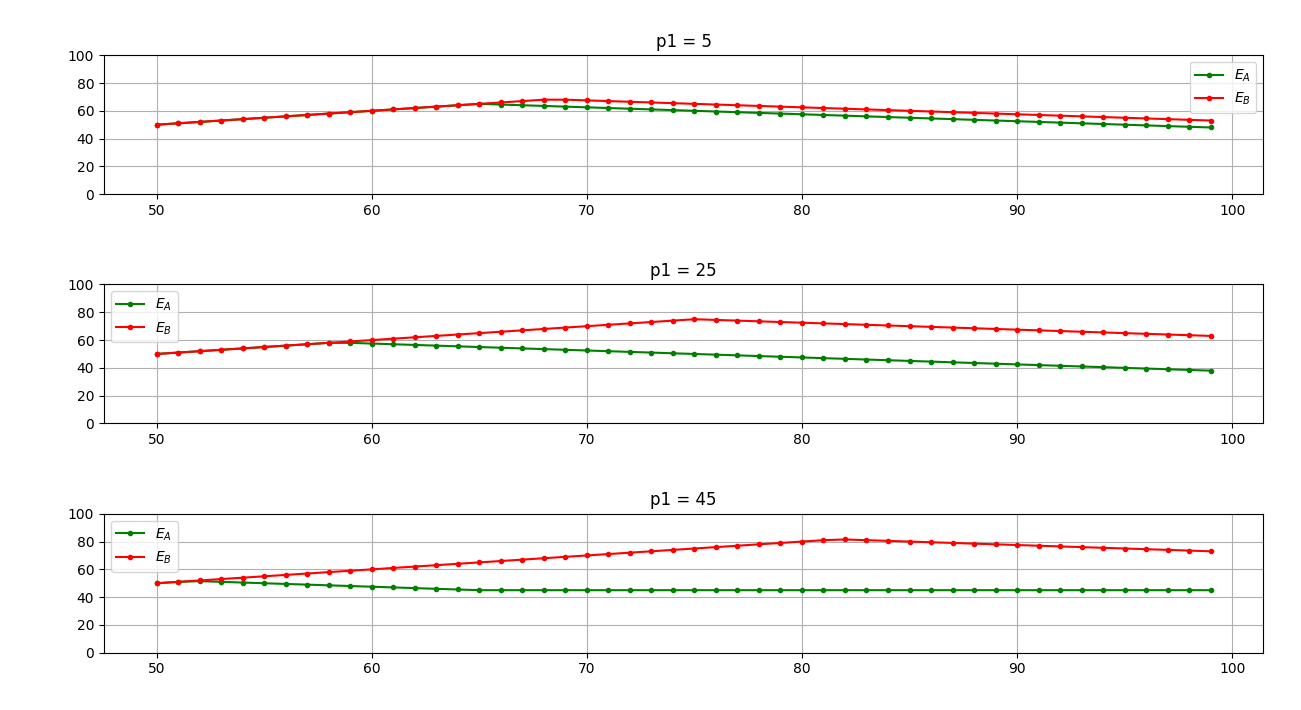
\includegraphics[width=\textwidth]{Images/GainedProfitp2SecondHalfWorld.png}
% \caption{Expected profits for different cases of $r$}
% \label{figures:1D,partial,FullInfo,B case}
% \end{figure}

% Note that in practice, this is the same response for $S_\opp = \gf$, so we can say that either way, \rob's best response is to go toward $i_\opp$, regardless to $S_\opp$.

\paragraph{Partial Information - $i_\opp$ is known, $S_\opp$ is unknown - asymmetrical-Knowledge}
This case was much simpler: according to the full knowledge case, for either $S_\opp \in \lbrace \gn,\gf \rbrace$ the best response is to go towards $i_\opp$, which in this case, is known.

This result is interesting: what we show is, actually, that knowing the opponent' strategy does not count for anything. This result stands in contrast to what we found in the 2D similar case, as will be shown.

\paragraph{Partial Information - $i_\opp$ is unknown, $S_\opp$ is known - asymmetrical-Knowledge} \label{sections:1D unknown io known so}
In this case, we have yet been unsuccessful in proving the optimal strategy for \rob, maximizing its \fcc. We have constructed the expected \fcc functions for both $S_\opp = \gn$ and $S_\opp = \gf$ by checking each and different case for both options of available $S_\opp$s, and for all different ranges of optional $i_\opp$. An example for such plot is shown in figure \ref{figures:examples Sos utility}:

\begin{figure}
\begin{tikzpicture}[thick,framed]
%draw players
  \draw (0,0) -- (\len,0);
  \draw[snake=ticks,segment length=1cm] (0,0) -- (\len,0);
  \node[above] at (0,0) {$\textsc{0}$};% label the hinge
  \node[above] at (\len,0) {$\textsc{L+R}$};% label the hinge
  
  \filldraw[ball color=blue!80,shading=ball] (0.1*\len,0.5) circle
        (0.06cm) node[above]{$r$};% p1
  
  \filldraw[ball color=red!80,shading=ball] (0.8*\len,0.5) circle
        (0.06cm) node[above]{$o$};% p2
     
   % draw path
   \draw[->, blue] (0.1*\len,0.5) -- (0.0*\len,0.5)
	  	node[pos=0.7,above]{}; % path1 p2
   \draw[->, blue, dashed] (0.0*\len,0.4) -- (0.1*\len,0.4)
	  	node[pos=0.7,above]{}; % path1 p2
   \draw[-, green] (0.1*\len,0.4) -- (0.3*\len,0.4)
	  	node[pos=0.7,above]{}; % path1 p2
   \draw[->, blue] (0.3*\len,0.4) -- (0.55*\len,0.4)
	  	node[pos=0.7,above]{}; % path1 p2
   
   \draw[-, red, dashed] (0.8*\len,0.5) -- (\len,0.5)
	  	node[pos=0.5,above]{}; % path1 p1
   \draw[->, red, dashed] (\len,0.4) -- (0.55*\len,0.4)
	  	node[pos=0.5,above]{}; % path1 p1
   
   % draw axis
   \draw[<->] (0, -0.3) -- (0.45*\len, -0.3)
        node[pos=0.5,below]{$\textsc{L}$}; % Left hand
   \draw[<->] (0.45*\len, -0.3) -- (\len, -0.3)
        node[pos=0.5,below]{$\textsc{R}$}; % Right Hand
\end{tikzpicture}
\caption{An example for a single considered case. (Green is the extra part \rob is doing before \opp is reaching its initial position)}
\label{figures:examples Sos utility}
\end{figure}

Lemmas \ref{theorems: 1d unknown io so=GN}, \ref{theorems: 1d unknown io so=GF} are yet left to be prove, and  their utility functions are displayed (for correctness-seeing purposes) in figures \ref{figures:1d unkown Io So=GN} and \ref{figures:1d unkown Io So=GF}.
\begin{theorem} \label{theorems: 1d unknown io so=GN}
$\mathbb{E}[\fcc_\rob (S_\rob=\gf, S_\opp=\gn)] > \mathbb{E}[\fcc_\rob (S_\rob=\gn, S_\opp=\gn)]$
\end{theorem}
\begin{theorem} \label{theorems: 1d unknown io so=GF}
$\mathbb{E}[\fcc_\rob (S_\rob=\gf, S_\opp=\gf)] > \mathbb{E}[\fcc_\rob (S_\rob=\gn, S_\opp=\gf)]$
\end{theorem}

% For both cases, it is clear that $S_\rob = \gf$ yield higher $\mathbb{E}[\fcc]$ than $S_\rob = \gn$, the functions are displayed in figure \ref{figures:1d unkown Io So=GN} and figure \ref{figures:1d unkown Io So=GF}.

\begin{figure}
    \centering
    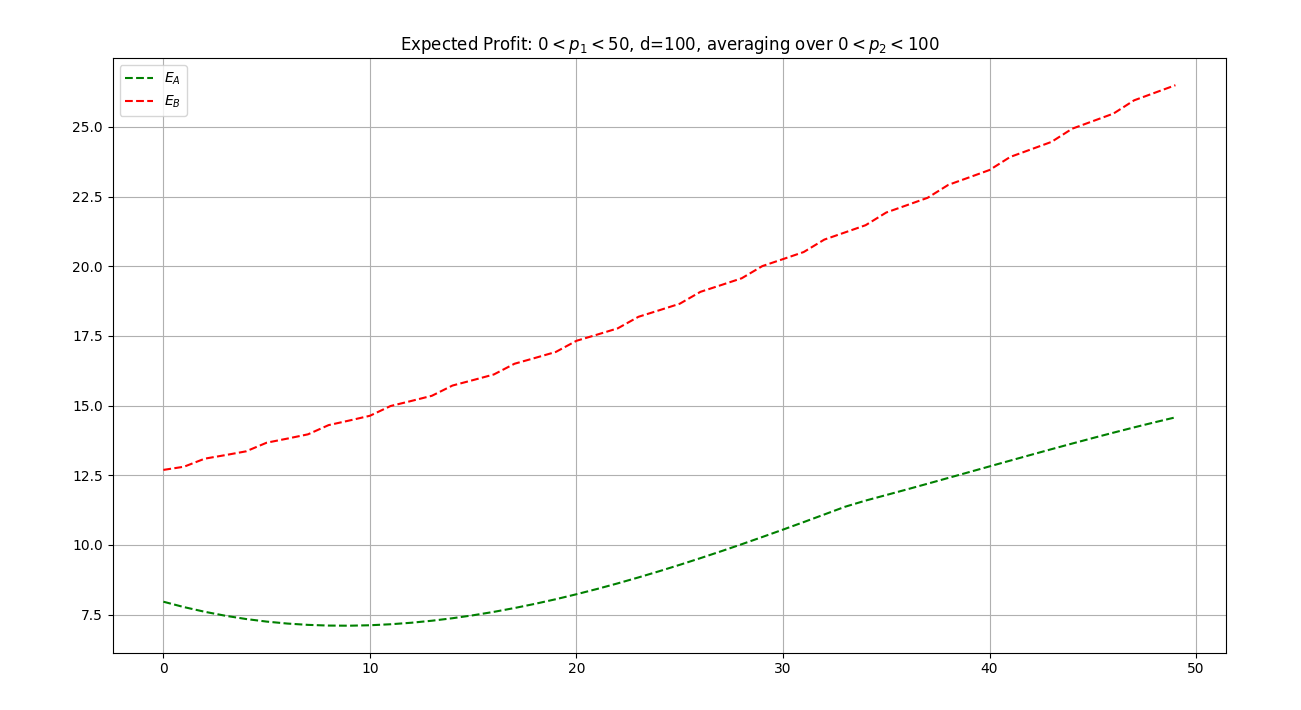
\includegraphics[width=\textwidth]{Images/E1_E2_p2A_abs.png}
    \caption{$i_\rob$ values vs. $\mathbb{E}[\fcc_\rob]$, averaging gained $\fcc_\rob$  $0<i_\opp<100$, $S_\opp=\gn$ \gn is green and \gf is red}
    \label{figures:1d unkown Io So=GN}
\end{figure}

\begin{figure}
    \centering
    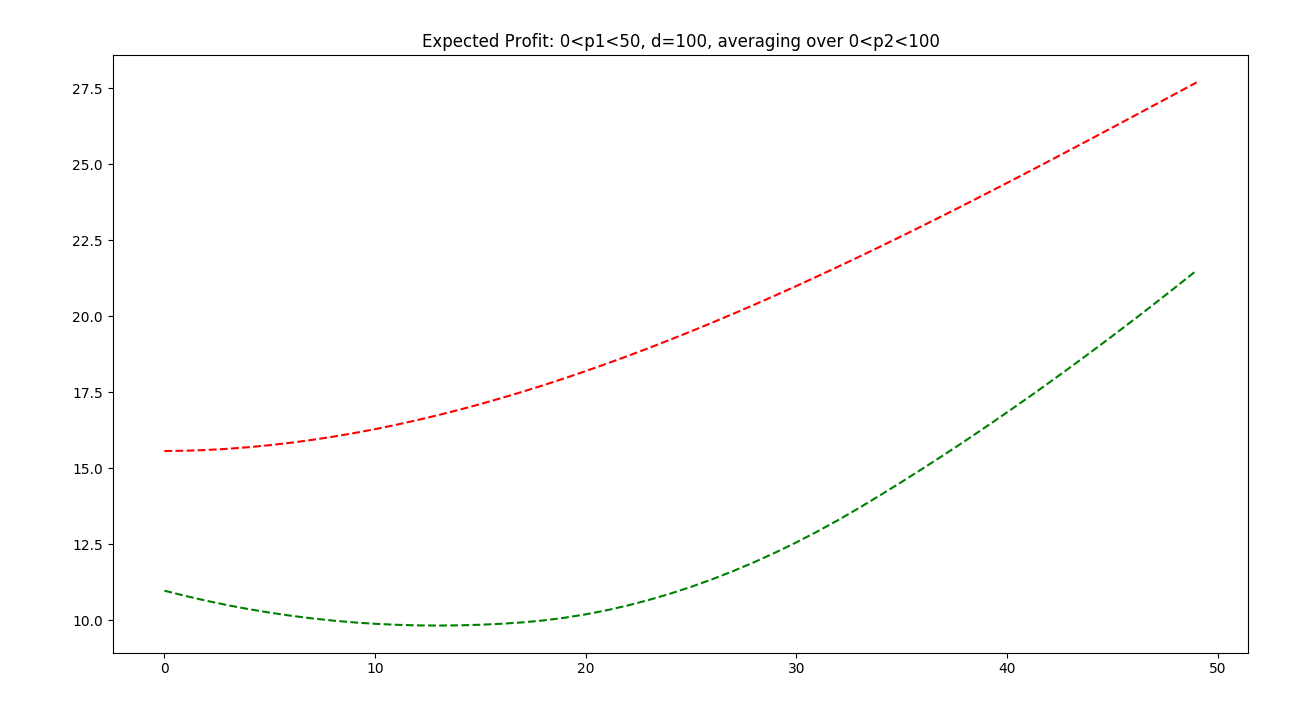
\includegraphics[width=\textwidth]{Images/E1_E2_w_wo_abs.png}
    \caption{$i_\rob$ values vs. $\mathbb{E}[\fcc_\rob]$, averaging gained $\fcc_\rob$  $0<i_\opp<100$, $S_\opp=\gf$ \gn is green and \gf is red}
    \label{figures:1d unkown Io So=GF}
\end{figure}

\paragraph{Zero Information - asymmetrical-Knowledge}
In this case, we started by proving Theorems \ref{theorems: 1D no info basic} and \ref{theorems: 1D not info not recognize}.
\begin{theorem} \label{theorems: 1D no info basic}
When $IM_\rob=\lbrace S_\emptyset, i_\emptyset \rbrace$, \rob's optimal strategy is obtained by $S_\rob = \gf$.
\end{theorem}
\begin{theorem} \label{theorems: 1D not info not recognize}
When $IM_\rob=\varnothing$, \rob's optimal strategy is obtained by $S_\rob = \gn$.
\end{theorem}

Figures \ref{figures:1d unkown Io So=GN} and \ref{figures:1d unkown Io So=GF}, demonstrate that \rob's optimal strategy is $S_\rob=\gf$, but it will play it only when $IM_\rob \neq \varnothing$, otherwise \rob only wants to minimize its running time. This leads us to the conclusion described in Theorem \ref{theorems: utility of no information}.

\begin{theorem}\label{theorems: utility of no information}
$IM=\lbrace S_\emptyset, i_\emptyset \rbrace$ yields better results than $IM_\rob=\varnothing$.
\end{theorem}

Which means that in the zero-information, asymmetrical case, it is best to play $S_\rob=\gf$, and it is better than playing as if \opp is not exists. 

\subsection{2D World}
Same as before, we start by considering different information models: either \rob is given, or not, the initial location of \opp, $i_\opp$, and its strategy, $S_\opp$. Then, assuming a very basic behavior, where only \rob is aware of \opp's existence, and it must decide its strategy before the game begins, we tried to find the best strategy $S_\rob$ for \rob, given the information model.
Given this information model, we start by considering the asymmetric case in which only \rob is aware of \opp. Hence, we aim at determining the optimal strategy $S_\rob$ for \rob, based on the information models.

\subsubsection{Information Models}
Also here, we considered the four information models described in Section \ref{sections:1D intro}
% There are 4 basic information model: 
% \begin{enumerate}
% \item \textbf{Full information} - $i_\opp$ is known, $S_\opp$ is known
% \item \textbf{Zero-Information} - $i_\opp$ is known, $S_\opp$ is unknown
% \item \textbf{Partial Information} -  $i_\opp$ is unknown, $S_\opp$ is known
% \item \textbf{Partial Information} - $i_\opp$ is unknown, $S_\opp$ is unknown
% \end{enumerate}

\paragraph{Full Information - asymmetrical-Knowledge}

In the full information case we present a new algorithm, \gipc (\ref{algorithms: gipc}) that maximizes the \fcc target function.
The algorithm is presented in \ref{algorithms: gipc}:
\begin{algorithm}
\begin{algorithmic}
	\STATE $i_p^{S_\rob S_\opp} \leftarrow $ Find Interception Point between $S_\rob$ and $S_\opp$
    \STATE GoTo $i_p^{S_\rob S_\opp}$, precede \opp by one step
    \LOOP
    	\IF {Cell $c_i$ \NOT Covered already}
        	\STATE GoTo $S_\opp(c_i)$
        \ENDIF
    \ENDLOOP
  
\end{algorithmic}
\caption{GIPC\label{algorithms: gipc}}
\end{algorithm}

\begin{theorem}
\gipc is correct, complete and optimal, and on a rectangular grid of size $m\times n$ it yields \[\mathbb{E}[\fcc] = m\cdot n-\frac{\left(m+1\right)\left(m-1\right)}{3m}-\frac{\left(n+1\right)\left(n-1\right)}{3n}\]
\end{theorem}

% Lastly, we do experiments. We start by running code simulations, to check that our algorithm is correct, that it is indeed the most preferable strategy, and that it does yield the computed expected \fcc.
% Then, we'll do realistic simulations using ROS, to see that $GIPC$ works correctly and as expected under real-world constraints, also.

\paragraph{Zero Information - asymmetrical-Knowledge}
In the zero-information case, \rob knows neither $i_\opp$ nor $S_\opp$. In fact, in this information model, \rob knows about \opp only that it exists.

We then introduce the \cros algorithm(\ref{algorithms: cros}), proven theoretically (Theorem \ref{theorems: cros correctness and optimalty}) that it is the best strategy to play, and de-facto, knowing an opponents exists in the world, does not give \rob any advantage. Lastly, we prove the resulted $\mathbb{E}[\fcc]$ in Theorem \ref{cross efcc}.

\begin{algorithm}
\begin{algorithmic}
	\STATE Choose $S_\rob \in \mathcal{S}$ in random.
    \STATE $c_i \leftarrow i_\rob$
    \LOOP
    	\STATE $c_i \leftarrow S_\rob(c_i)$
    \ENDLOOP
  
\end{algorithmic}
\caption{\cros\label{algorithms: cros}}
\end{algorithm}

\begin{theorem} \label{theorems: cros correctness and optimalty}
\cros is correct, complete and when $IM_\rob=\lbrace S_\emptyset, i_\emptyset \rbrace$, is optimal.
\end{theorem}

\begin{theorem} \label{cross efcc}
Given $IM_\rob=\lbrace S_\emptyset, i_\emptyset \rbrace$, then $\mathbb{E}[\fcc_\rob(S_\rob=\cros)]=\frac{N+1}{2}$.
\end{theorem}

% Lastly, we do experiments. We perform simulations, showing our claims about the optimality of playing \cros (in this specific information model), and about the given expected \fcc it yields, are correct. 
% Lastly, we do hard experiments using ROS, to show that indeed, the expected \fcc when $S_\rob=\cros$ with no other information, and averaging over different strategies and initial positions, are indeed what we claim, and that it works under real-world constraints.

\paragraph{Partial Information - $i_\opp$ is unknown, $S_\opp$ is known - asymmetrical-Knowledge} 


In this case, where \rob knows $S_\opp$, but not $i_\opp$, we examine whether \rob can achieve anything better than playing \cros, given that is is given more information: According to Theorem \ref{theorems: 2d max fcc unknown io} ,\rob cannot. The best $\mathbb{E}[\fcc]$ \rob can achieve is $\frac{N+1}{2}$.

We present a new strategy, \coos(\ref{coos algorithm}), where $S_\rob$ is set to be the opponents strategy, $S_\opp$. 
\begin{algorithm}
\begin{algorithmic}
	\STATE Choose $S_\rob \leftarrow S_\opp$
    \STATE $c_i \leftarrow i_\rob$
    \LOOP
    	\STATE $c_i \leftarrow S_\rob(c_i)$
    \ENDLOOP
  
\end{algorithmic}
\caption{\coos\label{coos algorithm}}
\end{algorithm}

We prove in Theorem \ref{theorems: coos stupid}, sadly, that this does not increase the expected \fcc, as we hoped for.
\begin{theorem} \label{theorems: coos stupid}
 When $IM_\rob=\lbrace S_\opp , i_\emptyset \rbrace$, then \[\mathbb{E}[\fcc_\rob(\coos, S_\opp)]=\frac{N+1}{2}\]
\end{theorem}

We then prove the more important Theorem \ref{theorems: 2d max fcc unknown io}, which brings a surprising result: the knowledge about $S_\opp$ is irrelevant to \opp, and can not help him achieve anything better than random-like results.

\begin{theorem}\label{theorems: 2d max fcc unknown io}
When $IM_\rob=\lbrace S_\opp , i_\emptyset \rbrace$, then \[\max \lbrace \mathbb{E}[\fcc_\rob(S_\rob, S_\opp)]\rbrace=\mathbb{E}[\fcc_\rob(S_\rob, S_\opp)]=\frac{N+1}{2}\]
\end{theorem}
\begin{proof}

\end{proof}


\paragraph{Partial Information - $S_\opp$ is unknown, $i_\opp$ is known - asymmetrical Knowledge} 
This is the last information model we want in the asymmetrical knowledge case. In this case, we have yet been unable to prove superiority of any better-than-random strategy.
Checking our simulations, we know that indeed, there are some strategies that yield better results; That is, there are some $S^{better}_{\opp}\in \mathcal{S}$ that yield $\mathbb{E}[\fcc(S_\opp=S^{better}_{\opp})] > \frac{N+1}{2}$, but we did not yet manage to prove what character made them better than other. So we know such better strategies exists.

We did prove, in Theorem \ref{theorems: 2d known io unknown so} is that playing the same as your opponent is irrelevant.
\begin{theorem} \label{theorems: 2d known io unknown so}
When $IM_\rob = \lbrace S_\emptyset, i_o \in \w \rbrace$, then \[\mathbb{E}[\fcc_\rob(S_\rob=S_\opp, S_\opp)] = \mathbb{E}[\fcc_\rob(S_\rob=\cros, S_\opp)] = \frac{N+1}{2}\]
\end{theorem}


% This is the last information model we want in the asymmetrical Knowledge case. Here, \rob gets the initial position of \opp, but not its strategy.
% As was shown before, the key component to improving the \fcc criterion is to know $i_\opp$. So, what do we know:
% Right now, we stand in a very interesting, even if a little frustrating: We checked and saw that \rob has better-than-other strategies to play when the initial position $i_\opp$ is known (and set) and averaging over different strategies. But we do not know what are the criteria for a good or bad strategy.

This part is remained to be investigated. 

\section{Work Plan}
The next steps in our work will be:
\begin{enumerate}
\item Analyze the symmetric game in 1D world.

Up to this point, we considered the asymmetric version of our problem, where \rob knows or does not know {\opp}'s existence, strategy and initial position, and \opp acts as if it is alone, and it only goal is to cover as fast as possible.
A more realistic model is the symmetric knowledge model, where \opp knows as much about \rob as \rob knows about \opp.

We will go though the four information models available, and will try to find the best strategy for \rob, taking in consideration $S_\opp$, which now will be more complex. Then, we will try to give numerical analyzing about the given \fcc. At the end, the same way as before, we check our results using simple and realistic simulations in order to verify our results.

\item Analyze the symmetric game in 2D world.
As mentioned above for 1D, we will do the same for 2D.
We will start by considering the offline problem, where \rob and \opp need to choose, in advance, what they should do, considering that now \opp knows about \rob (either mere existence, initial position, strategy, or a combination of above).
Going through the four information models, we will try to find what is  best strategy $S_\rob$ for \rob. 
After that, we will check to see if when considering a finite number of strategies, we are to find some Nash-Equilibrium, where both players have the same information model, and they both prefer to use the same strategy, each of them prefer to stick with its strategy, considering the other one is doing the same. We will then analyze the results using game-theory tools.

\item Research the fourth information model in 2D asymmetrical world.

As mentioned above, we saw that there are some strategies that yield better-than-random result. 
We would like to try and find some characteristics which indicates a strategy would be better than others.

\item Implements realistic simulation to 1D and 2D worlds for different cases of information models.

Finally, we would like and test our claims and theorems under real-world constraints. We will use ROS/Gazebo in order to implement the main algorithms and behaviors mentioned above, and check that they are indeed working correctly.
We would like to know what changes, if any, are needed in order for them to work correctly.

\end{enumerate}


\bibliographystyle{abbrv}
\bibliography{SharedParts/refs}

\end{document}
